\definecolor{shadecolor}{RGB}{190,190,190}

\section{Benchmarking}
L'architecture adoptée pour notre application web est l'architecture client-serveur, où le serveur ne gère pas l’affichage mais seulement envoyer des données brutes à afficher, et toute la génération des écrans et la gestion des interactions avec l’utilisateur doivent être gérées côté client, c’est-à-dire dans le navigateur.\\
\begin{figure}[h!]  
 \centering
    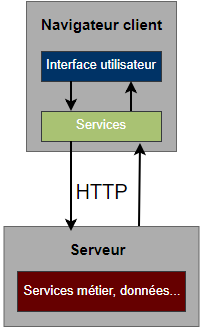
\includegraphics[width=0.26\textwidth]{chapitre3/Figures/client-serveur.png}
  \caption{L'architecture technique de l'application}
\end{figure}
\newpage
L’adoption de cette architecture nécessite de trouver les technologies adéquates pour développer le Back-end ainsi que le Front-end.  Alors, une étude comparative est jugée nécessaire pour sélectionner un framework (Front-end, Back-end) qui répond plus aux besoins et critères sous-mentionnés.
\subsubsection*{Critères de comparaison}
La détermination des critères sur lesquels une étude comparative se base, s’avère indispensable pour atteindre les résultats attendus. Pour cela, des réunions avec notre encadrant interne pour la spécification des critères étaient jugées nécessaires dans cette étude. Et en voici les critères de comparaison résultant ci-dessous :\\
Les critères de comparaison des frameworks \textbf{Back-end :}
\begin{itemize}[label=\textbullet]
  \item Communauté
  \item Encadrement au sein de la société
  \item Documentation
  \item Facilité de configuration
  \item Facilité de prise en main
\end{itemize}
Les critères de comparaison des frameworks \textbf{Front-end :}
\begin{itemize}[label=\textbullet]
  \item Communauté
  \item Documentation
  \item Facilité de prise en main
  \item Open Source
  \item Support du navigateur
\end{itemize}
%%% back END
\subsection{Etude comparative des frameworks Back-end}
Le tableau suivant présente l'ensemble des frameworks Back-end étudié durant cette étude comparative : \newpage
%tableau
\begin{table}[!h]
\begin{tabular}{|>{\columncolor{shadecolor}}p{2.5cm}|p{9cm}|}
\hline
Spring Boot&Spring est un framework bien connu des développeurs Java pour les nombreuses fonctionnalités qu’il apporte sur les aspects web, sécurité, batch ou encore accès aux données dans le cadre du développement d’une application Web\\
\hline
Java EE&La plateforme Java EE est un ensemble de spécifications coordonnées et pratiques qui permettent des solutions pour le développement, le déploiement, et de la gestion des applications multi-tiers centralisées sur un serveur\\
\hline
.NET&.NET est un framework de programmation créé par Microsoft que les développeurs peuvent utiliser pour créer des applications Web\\
\hline
\end{tabular}
\centering \caption{Frameworks Back-end étudiés} \label{TablePR}
\end{table}
\subsubsection*{Résultat de l'étude}
Suite à la détermination des critères de ce benchmarking, la phase qui suit est la phase sur laquelle nous nous baserons pour choisir l’un des frameworks Back-end. Pour cela, une étude de chaque framework est nécessaire pour l’attribution des notes d’évaluation. Le tableau suivant présente le résultat de cette étude :
\begin{table}[!h]
\begin{tabular}{|>{\columncolor{shadecolor}}c|c|c|c|}
\cline{2-4}
\rowcolor{shadecolor}\multicolumn{1}{c|}{\backslashbox[70mm]{Critère}{Framework}}&Spring Boot&Java EE&.NET\\
\hline
Communauté&Bien&Bien&Moyen\\
\hline
Encadrement au sein de la société&Bien&Bien&Faible\\
\hline
Documentation&Moyen&Moyen&Bien\\
\hline
Facilité de configuration&Moyen&Faible&Bien\\
\hline
Facilité de prise en main&Bien&Moyen&Moyen\\
\hline
\end{tabular}
\centering \caption{Comparatif entre les technologies du Back-end} \label{TablePR}
\end{table}

\subsubsection*{Choix du framework}
Le choix du framework est basé sur les notes attribuées à chaque framework pour chaque critère. Le schéma suivant est une représentation graphique qui montre la synthèse de cette étude et permet de juger le framework qui répond au plus à ces critères.\newpage
\begin{figure}[h!]  
 \centering
    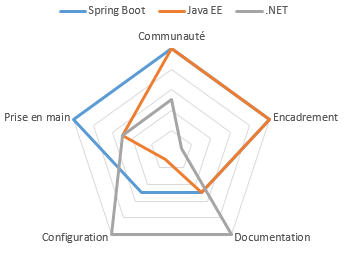
\includegraphics[width=0.7\textwidth]{chapitre3/Figures/benchBack.png}
  \caption{Synthèse de l'étude comparative sous forme de graphe}
\end{figure}
D’après ce graphe, Spring Boot est jugé le framework qui répond plus aux besoins et critères spécifiés.

%%% front END
\subsection{Etude comparative des frameworks Front-end}
Le tableau suivant présente l'ensemble des frameworks Front-end étudié durant cette étude comparative : 
%tableau
\begin{table}[!h]
\begin{tabular}{|>{\columncolor{shadecolor}}p{2.5cm}|p{9cm}|}
\hline
Angular&Angular est un framework JavaScript MVVM superheroique, fondé en 2009, qui est génial pour la création d'applications web hautement interactives.\\
\hline
Ember.js&Ember.js est un cadriciel (framework) open-source JavaScript tourné vers les applications web.  Il s'appuie sur une architecture de type MVC (modèle-vue-contrôleur). Il permet aux développeurs de créer des applications single-page\\
\hline
React&ReactJS est une bibliothèque JavaScript, ouverte par Facebook en 2013, qui permet la création d'applications web où les données sont changeables sur une base régulière\\
\hline
Vue.js&Vue.js est un framework JavaScript, lancé en 2013, qui convient parfaitement à la création d'interfaces utilisateur hautement adaptables et d'applications Single-page sophistiquées\\
\hline
\end{tabular}
\centering \caption{Frameworks Front-end étudiés} \label{TablePR}
\end{table}
\subsubsection*{Résultat de l'étude}
Suite à la détermination des critères de ce benchmarking, la phase qui suit est la phase sur laquelle nous nous baserons pour choisir l’un des frameworks Front-end. Pour cela, une étude de chaque framework est nécessaire pour l’attribution des notes d’évaluation. Le tableau suivant présente le résultat de cette étude :
\begin{table}[!h]
\begin{tabular}{|>{\columncolor{shadecolor}}c|c|c|c|c|}
\cline{2-4}
\rowcolor{shadecolor}\multicolumn{1}{c|}{\backslashbox{Critère}{Framework}}&Angular& Ember.js&React&Vue.js\\
\hline
Communauté&Bien&Faible&Bien&Faible\\
\hline
Documentation&Bien&Moyen&Faible&Moyen\\
\hline
Facilité de prise en main&Moyen&Faible&Moyen&Bien\\
\hline
Open Source&Oui&Oui&Oui&Oui\\
\hline
Support du navigateur&Tous&Tous&Tous&Tous\\
\hline
\end{tabular}
\centering \caption{Comparatif entre les technologies du Front-end} \label{TablePR}
\end{table}

\subsubsection*{Choix du framework}
Le choix du framework est basé sur les notes attribuées à chaque framework pour chaque critère. Le schéma suivant est une représentation graphique qui montre la synthèse de cette étude et permet de juger le framework qui répond au plus à ces critères.
\begin{figure}[h!]  
 \centering
    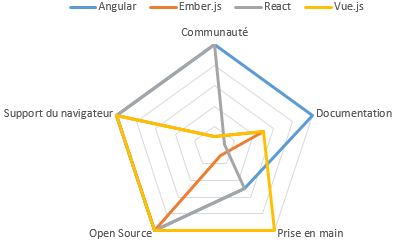
\includegraphics[width=0.7\textwidth]{chapitre3/Figures/benchFront.png}
  \caption{Synthèse de l'étude comparative sous forme de graphe}
\end{figure}
\\
D’après ce graphe, Angular est jugé le framework qui répond plus aux besoins et critères spécifiés.



